
\section{Specific Structure of VAE}

\subsection{Encoder}

\[
(\mu, \sigma^2) = \text{EncoderNetwork}_\phi(x)
\]
\[
q_\phi(z|x) = \mathcal{N}(z | \mu, \sigma^2 I)
\]

The parameters \( \mu \) and \( \sigma \) are technically neural networks because they are outputs of \( \text{EncoderNetwork}_\phi(\cdot) \).

\vspace{0.3cm}

We denote them as:
\[
\mu = \mu_\phi(x) \quad \text{and} \quad \sigma^2 = \sigma^2_\phi(x).
\]

Given the \(\ell\)-th training sample \( x^{(\ell)} \), the latent variable \( z^{(\ell)} \) is sampled as:
\[
z^{(\ell)} \sim \mathcal{N} \left( z \mid \mu_\phi(x^{(\ell)}), \sigma^2_\phi(x^{(\ell)})I \right).
\]

\subsection{Sampling with Reparameterization Trick}

From the Gaussian, we draw a sample \( z^{(\ell)} \):
\[
z^{(\ell)} = \mu_\phi(x^{(\ell)}) + \sigma_\phi(x^{(\ell)}) \epsilon, \quad \epsilon \sim \mathcal{N}(0, \textbf{I}).
\]
\begin{figure}
    \centering
    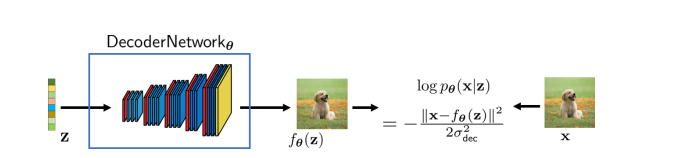
\includegraphics[width=1\linewidth]{sec/anh02.png}
    \caption{Implementation of a VAE encoder. The neural network takes \( x \) and estimates \( \mu_\phi \) and \( \sigma^2_\phi \).}
    \label{fig:vae_encoder}
\end{figure}

\subsection{KL Divergence of Two Gaussians}
\begin{mdframed}
\textbf{Theorem 1.3: KL-Divergence of Two Gaussians} ~\cite{chan2025tutorial}

The KL divergence for two \(d\)-dimensional Gaussian distributions \( \mathcal{N}(\mu_0, \Sigma_0) \) and \( \mathcal{N}(\mu_1, \Sigma_1) \) is:
\begin{align*}
D_{\text{KL}}\left(\mathcal{N}(\mu_0, \Sigma_0) \parallel \mathcal{N}(\mu_1, \Sigma_1)\right) 
&= \frac{1}{2} \Big[ \text{Tr}(\Sigma_1^{-1} \Sigma_0) - d \\
&\quad + (\mu_1 - \mu_0)^T \Sigma_1^{-1} (\mu_1 - \mu_0) \\
&\quad + \log \frac{\det \Sigma_1}{\det \Sigma_0} \Big].
\end{align*}
\end{mdframed}

\subsection{KL Divergence in VAE}

\textbf{Substituting Specific Distributions:}
\[
\mu_0 = \mu_\phi(x), \quad \Sigma_0 = \sigma_\phi^2(x) \textbf{I}, \quad \mu_1 = 0, \quad \Sigma_1 = \textbf{I}.
\]

\textbf{Simplified KL Divergence:}
\[
D_{\text{KL}}\left(q_\phi(z \mid x) \parallel p(z)\right) = 
\frac{1}{2} \Big[ 
\sigma_\phi^2(x) d - d + \|\mu_\phi(x)\|^2 - 2 \log \sigma_\phi(x) 
\Big].
\]

Here, \(d\) is the dimension of the latent vector \(z\).

\subsection{Decoder}

The decoder network, \( \text{DecoderNetwork}_\theta(\cdot) \), maps a latent variable \( z \) to a generated image or data point:
\[
f_\theta(z) = \text{DecoderNetwork}_\theta(z).
\]

The likelihood of the data given the latent variable, \( p_\theta(x \mid z) \), is assumed to follow a Gaussian distribution:
\[
p_\theta(x \mid z) = \mathcal{N}(x \mid f_\theta(z), \sigma_{\text{dec}}^2 I),
\]
where \( \sigma_{\text{dec}} \) is a hyperparameter that determines the variance of the Gaussian distribution. 

\textbf{Reparameterization Trick:} The generated data point \( \widehat{x} \) can be sampled as:
\[
\widehat{x} = f_\theta(z) + \sigma_{\text{dec}} \epsilon, \quad \epsilon \sim \mathcal{N}(0, I).
\]

\subsection*{Log-Likelihood of \( p_\theta(x \mid z) \)}

The log-likelihood of the data given \( z \) can be expressed as:
\begin{align*}
  \log p_\theta(x|z) &= \log \mathcal{N}(x \mid f_\theta(z), \sigma_{\text{dec}}^2 I) \\
  &= - \frac{\|x - f_\theta(z)\|^2}{2 \sigma_{\text{dec}}^2} 
  - \frac{d}{2} \log(2\pi \sigma_{\text{dec}}^2),
\end{align*}
where \( d \) is the dimensionality of \( x \). 

The constant term \( -\frac{d}{2} \log(2\pi \sigma_{\text{dec}}^2) \) does not depend on the model parameters \( \theta \) and can be ignored during optimization.

\vspace{10pt}
\textbf{Explanation:}
\begin{itemize}
    \item \( f_\theta(z) \): The deterministic mapping from \( z \) to the mean of the Gaussian distribution.
    \item \( \sigma_{\text{dec}}^2 \): Variance of the Gaussian distribution, controlling how tightly \( x \) is expected to cluster around \( f_\theta(z) \).
\end{itemize}


\subsection{VAE Training: Optimization Objective}

To train a VAE, we need to solve the optimization problem ~\cite{chan2025tutorial}:
\[
\arg\max_{\theta, \phi} \sum_{x \in \mathcal{X}} \text{ELBO}_{\phi, \theta}(x),
\]
where:
\[
\text{ELBO}_{\phi, \theta}(x) = \text{Reconstruction Term} + \text{KL Divergence Term}.
\]

\subsection*{Reconstruction Term}
\[
- \frac{1}{M} \sum_{m=1}^M 
\frac{\|x - f_\theta\left(\mu_\phi(x) + \sigma_\phi(x)\epsilon^{(m)}\right)\|^2}{2\sigma_\text{dec}^2}.
\]

\subsection*{KL Divergence Term}
\[
+ \frac{1}{2} \Big(\sigma_\phi^2(x)d - d + \|\mu_\phi(x)\|^2 - 2 \log \sigma_\phi(x) \Big).
\]

\subsection*{Explanation of Terms}
\begin{itemize}
    \item \( \mu_\phi(x) \): Mean output of the encoder.
    \item \( \sigma_\phi(x) \): Standard deviation output of the encoder.
    \item \( d \): Dimension of the latent variable \(z\).
\end{itemize}
